\chapter{Introduction}

The ecoMOD project is focused on creating sustainable, prefabricated housing units in partnership with local affordable housing organizations. These units are sustainable in that are environmentally responsive, with reduced energy, water, and maintenance costs compared to traditional housing stock. ecoMOD housing is aggressively affordable without cutting corners in construction, and strives to utilize the latest best practices in green, low-impact building and construction for a total cost of ownership that is markedly less than average. As a result, ecoOMOD housing has received numerous awards and accolades in the trade space\cite{Lau2013}.

\begin{figure}
\centering
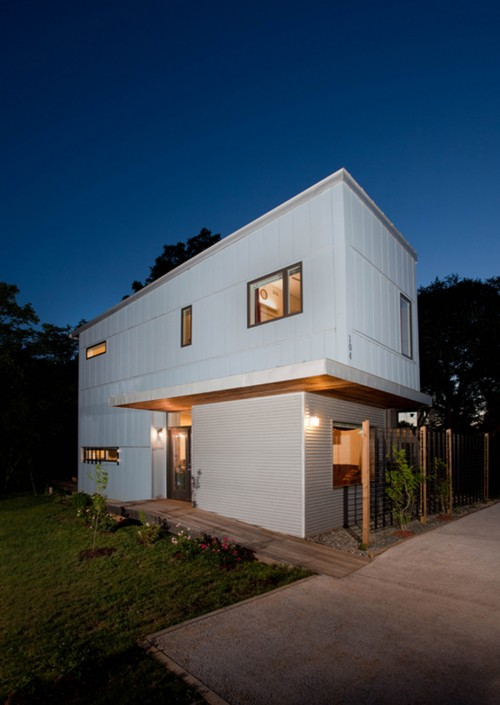
\includegraphics[width=0.3\linewidth]{./images/SFSmith_110602_8113-copy-500x705}
\caption{ecoMOD 4 in the evening\cite{Smith2011}}
\label{fig:SFSmith_110602_8113-copy-500x705}
\end{figure}

Historically, all ecoMOD housing has been extensively monitored and networked for reasons of evaluating building performance. These sensors monitor important information such as ambient temperature, humidity levels, air quality, and electricity use. This thesis is an extension of monitoring work that has been done continuously since the inception of the project, while introducing the foundations for future work in enabling environmental control. Three functional prototype sensors were developed as part of it: a soil moisture and temperature sensor for monitoring a ground source heat pump, an ambient light and temperature sensor, and an electronically controlled privacy shade.

Existing commercial monitoring solutions usually suffer the following problem: either they are excessively costly to install in the field, or are unreliable and difficult to integrate into existing data retrieval schemes. The ecoMOD project is no stranger to sensor deployments, having previously successfully opted to use expensive commercial solutions from vendors such as National Instruments or Onset Computers.

The sensors developed in this thesis leverage current open standards/software and wireless IPv6 networking to create easy-to-use, Internet ready devices that can present data seamlessly and securely over the web via a representational state transfer (REST)\cite{fielding2002principled} interface. The sensors can self-arrange themselves into ad-hoc wireless networks while consuming very little power by remaining in sleep mode until new data is acquired, with electronics that maintain a total bill of materials  cost of less than \$20 for boards made in single quantities. This level of performance is difficult to achieve with electronics in this price range, as usually more expensive micro-controllers running full real-time operating systems are needed. In addition, exposing the sensor data via HTTP means that no embedded programming knowledge is needed to provision new sensors, only basic familiarity with web services programming, and knowing how to flash a firmware image.

\section{Related Literature}

In general, existing sensor network deployments use incompatible physical and application layer communication interfaces. At the physical layer, the most popular of these are IEEE 802.15.4, Bluetooth low-energy, and IEEE 802.11. At the application layer, Zigbee, Z-Wave, WirelessHART, and CoAP all enjoy significant marketshare. However, more and more environmental monitoring systems are replacing their proprietary application layers with Internet communications.

There are a many reasons for this. In general, most wireless sensor data must be transported to a server or data repository via the Internet anyway. Therefore, having the sensor nodes exist natively on the Internet simplifies the data transmission process, and allows greater inter-operability between nodes who no longer need protocol bridges. The use of IP also allows the use of existing, mature tools for managing, provisioning, configuring, and debugging IP networks.  [37 IPv6 over low power wireless personal networks, RFC 4919 IETF Aug 2007]

For a great deal of time, Internet Protocol (IP) was not used because it was inappropriate for use in distributed wireless sensor networks. The protocol required too many computing resources as a proportion of microcontroller capability. However, the problem has been solved from two sides. First, the steady advance of Moore's Law has brought down the cost in power and money of embedding computing capability. Second, the IETF has defined several reduced-functionality subsets of IP that can be implmented on smaller computers. These are 802.15.4, ROLL, and CoAP. 

Hopefully, the adoption of IP for wireless sensor networks will speed their deployment and adoption. Communication compatibility between disparate devices will enable more competition between manufacturers, lower costs, and facilitate the creation of new services which span multiple sensor deployments. It will also allow the easy use of well-known Web technologies for aggregating and displaying sensor information.

TODO: Add paragraph or two addressing existing motes that run on Contiki or TinyOS.

\section{Principles of Sensing}
\subsection{Soil Moisture}

Zazueta, Fedro S., and Jiannong Xin. "Soil moisture sensors." Soil Sci 73 (1994): 391-401.

A ground-source heat pump (GSHP) was installed at ecoMOD 4. GSHPs transfer heat between the ground and a conditioned room or facility using electrical energy. Heat pump efficiency is inversely proportional to the temperature differential between the source and destination. As opposed to traditional electric air conditioners and heaters which use the ambient air temperature as the source, GSHPs source from the ground, whose temperature is approximately equal to the mean annual temperature year round, or around 50-60 degrees Fahrenheit, leading to generally better efficiency. GSHP installation and use disturbs the soil temperature, so in order to effectively calculate pump efficiency, the surrounding soil temperature and moisture content (which heavily determines the heat capacity of the surrounding soil) must be known.

Soil moisture can be measured in many different ways. However, only a few of these techniques lend themselves to automated electronic sensing, and the most common and widely available are based around either resistive or capacitive sensor methods. 

Capacitive methods involve measuring the dielectric capacitance between two electrodes. This is usually done by measuring the impedance at a specific frequency. The measured impedance is not linearly proportional to the amount of water present, and varies according to the composition and temperature of the measured soil. Therefore, for absolute precision, the sensor must be calibrated against a representative sample of soil and the temperature measured as well. When calibrated, the measurement is generally highly precise and can be measured instantaneously. Capacitive sensors are generally more expensive due to the more precise electronics required and calibration needed for accurate results.

\missingfigure{Irrometer Watermark Sensor}

Resistive techniques measure the DC resistance of a given volume of soil. The most common way of measuring this is by burying a porous gypsum block into the ground along with two electrodes, and allowing the block to come to hydrostatic equilibrium with the surrounding soil. This process usually takes two to three hours, which can also be seen after a rainstorm or other meteorological event. They are electronically simpler and cheaper to manufacture than capacitive sensors, which is an important consideration for their most common use, large-scale agricultural deployments. For many applications, individual block calibration can be ignored, since the gypsum medium is of a well-known composition and possesses a consistent resistivity. However, for long term measurement accuracy, the gypsum block must be continually recalibrated, as soil ions and salts can migrate into the gypsum block matrix, affecting the block resistance.

\missingfigure{Vegetronix}

\subsection{Ambient Humidity and Temperature}
